% !TEX TS-program = knitr
\documentclass[handout]{beamer}\usepackage[]{graphicx}\usepackage[]{color}
% maxwidth is the original width if it is less than linewidth
% otherwise use linewidth (to make sure the graphics do not exceed the margin)
\makeatletter
\def\maxwidth{ %
  \ifdim\Gin@nat@width>\linewidth
    \linewidth
  \else
    \Gin@nat@width
  \fi
}
\makeatother

\definecolor{fgcolor}{rgb}{0.345, 0.345, 0.345}
\newcommand{\hlnum}[1]{\textcolor[rgb]{0.686,0.059,0.569}{#1}}%
\newcommand{\hlstr}[1]{\textcolor[rgb]{0.192,0.494,0.8}{#1}}%
\newcommand{\hlcom}[1]{\textcolor[rgb]{0.678,0.584,0.686}{\textit{#1}}}%
\newcommand{\hlopt}[1]{\textcolor[rgb]{0,0,0}{#1}}%
\newcommand{\hlstd}[1]{\textcolor[rgb]{0.345,0.345,0.345}{#1}}%
\newcommand{\hlkwa}[1]{\textcolor[rgb]{0.161,0.373,0.58}{\textbf{#1}}}%
\newcommand{\hlkwb}[1]{\textcolor[rgb]{0.69,0.353,0.396}{#1}}%
\newcommand{\hlkwc}[1]{\textcolor[rgb]{0.333,0.667,0.333}{#1}}%
\newcommand{\hlkwd}[1]{\textcolor[rgb]{0.737,0.353,0.396}{\textbf{#1}}}%
\let\hlipl\hlkwb

\usepackage{framed}
\makeatletter
\newenvironment{kframe}{%
 \def\at@end@of@kframe{}%
 \ifinner\ifhmode%
  \def\at@end@of@kframe{\end{minipage}}%
  \begin{minipage}{\columnwidth}%
 \fi\fi%
 \def\FrameCommand##1{\hskip\@totalleftmargin \hskip-\fboxsep
 \colorbox{shadecolor}{##1}\hskip-\fboxsep
     % There is no \\@totalrightmargin, so:
     \hskip-\linewidth \hskip-\@totalleftmargin \hskip\columnwidth}%
 \MakeFramed {\advance\hsize-\width
   \@totalleftmargin\z@ \linewidth\hsize
   \@setminipage}}%
 {\par\unskip\endMakeFramed%
 \at@end@of@kframe}
\makeatother

\definecolor{shadecolor}{rgb}{.97, .97, .97}
\definecolor{messagecolor}{rgb}{0, 0, 0}
\definecolor{warningcolor}{rgb}{1, 0, 1}
\definecolor{errorcolor}{rgb}{1, 0, 0}
\newenvironment{knitrout}{}{} % an empty environment to be redefined in TeX

\usepackage{alltt}
\newcommand{\answers}{1}

\usetheme{Marburg}
\setbeamertemplate{navigation symbols}{} 
\setbeamertemplate{footline}
{
  \leavevmode%
  \hbox{%
  \begin{beamercolorbox}[wd=.333333\paperwidth,ht=2.25ex,dp=1ex,center]{author in head/foot}%
    \usebeamerfont{author in head/foot} $\ $ \insertshortauthor%~~\beamer@ifempty{\insertshortinstitute}{}{(\insertshortinstitute)}
  \end{beamercolorbox}%
  \begin{beamercolorbox}[wd=.333333\paperwidth,ht=2.25ex,dp=1ex,center]{title in head/foot}%
    \usebeamerfont{title in head/foot} \insertinstitute
  \end{beamercolorbox}%
  \begin{beamercolorbox}[wd=.333333\paperwidth,ht=2.25ex,dp=1ex,right]{date in head/foot}%
    \usebeamerfont{date in head/foot}\insertshortdate{}\hspace*{2em}
    \insertframenumber{} / \inserttotalframenumber\hspace*{2ex} 
  \end{beamercolorbox}}%
  \vskip0pt%
}

\usepackage{amsmath}
\usepackage{caption}
\usepackage{color}
\usepackage{enumerate}
\usepackage{listings}
\usepackage{hyperref}
\usepackage{mathrsfs}
\usepackage{natbib}
\usepackage{url}

\providecommand{\all}{\ \forall \ }
\providecommand{\bs}{\backslash}
\providecommand{\e}{\varepsilon}
\providecommand{\E}{\ \exists \ }
\providecommand{\lm}[2]{\lim_{#1 \rightarrow #2}}
\providecommand{\m}[1]{\mathbb{#1}}
\providecommand{\nv}{{}^{-1}}
\providecommand{\ov}[1]{\overline{#1}}
\providecommand{\p}{\newpage}
\providecommand{\q}{$\quad$ \newline}
\providecommand{\rt}{\rightarrow}
\providecommand{\Rt}{\Rightarrow}
\providecommand{\vc}[1]{\boldsymbol{#1}}
\providecommand{\wh}[1]{\widehat{#1}}

\hypersetup{colorlinks,linkcolor=,urlcolor=blue}
\numberwithin{equation}{section}

\definecolor{dkgreen}{rgb}{0,0.6,0}
\definecolor{gray}{rgb}{0.5,0.5,0.5}
\definecolor{mauve}{rgb}{0.58,0,0.82}

\lstset{ 
  language=C,                % the language of the code
  basicstyle= \footnotesize,           % the size of the fonts that are used for the code
  numberstyle= \tiny \color{white},  % the style that is used for the line-numbers
  stepnumber=2,                   % the step between two line-numbers. 
  numbersep=5pt,                  % how far the line-numbers are from the code
  backgroundcolor=\color{white},      % choose the background color. You must add \usepackage{color}
  showspaces=false,               % show spaces adding particular underscores
  showstringspaces=false,         % underline spaces within strings
  showtabs=false,                 % show tabs within strings adding particular underscores
  frame=lrb,                   % adds a frame around the code
  rulecolor=\color{black},        % if not set, the frame-color may be changed on line-breaks within not-black text 
  tabsize=2,                      % sets default tabsize to 2 spaces
  captionpos=t,                   % sets the caption-position 
  breaklines=true,                % sets automatic line breaking
  breakatwhitespace=false,        % sets if automatic breaks should only happen at whitespace
  %title=\lstname,                   % show the filename of files included with \lstinputlisting;
  keywordstyle=\color{blue},          % keyword style
  commentstyle=\color{gray},       % comment style
  stringstyle=\color{dkgreen},         % string literal style
  escapeinside={\%*}{*)},            % if you want to add LaTeX within your code
  morekeywords={*, ...},               % if you want to add more keywords to the set
  xleftmargin=0.053in, % left horizontal offset of caption box
  xrightmargin=-.03in % right horizontal offset of caption box
}

%\DeclareCaptionFont{white}{\color{white}}
%\DeclareCaptionFormat{listing}{\parbox{\textwidth}{\colorbox{gray}{\parbox{\textwidth}{#1#2#3}}\vskip-0.05in}}
%\captionsetup[lstlisting]{format = listing, labelfont = white, textfont = white}
%For caption-free listings, comment out the 3 lines above and uncomment the 2 lines below.
 \captionsetup{labelformat = empty, labelsep = none}
 \lstset{frame = single}



\title{Inference for Simple Linear Regression (Ch. 9.1)}
\author{Yifan Zhu}
\date{}
\institute{Iowa State University}
\IfFileExists{upquote.sty}{\usepackage{upquote}}{}
\begin{document}

\begin{frame}
\titlepage
 \end{frame}
 
 \AtBeginSection[]
{
   \begin{frame}
       \frametitle{Outline}
       \tableofcontents[currentsection]
   \end{frame}
}

\section{A Review of Simple Linear Regression (Ch. 4)}

\begin{frame}[fragile]
\frametitle{\small Pressing pressures and specimen densities for a ceramic compound}
\scriptsize
A mixture of $\text{Al}_2\text{O}_3$, polyvinyl alcohol, and water was prepared, dried overnight, crushed, and sieved to obtain 100 mesh size grains. These were pressed into cylinders at pressures from 2,000 psi to 10,000 psi, and cylinder densities were calculated. 

% latex table generated in R 3.5.2 by xtable 1.8-3 package
% Tue Apr 07 11:42:00 2020
\begin{table}[ht]
\centering
\begin{tabular}{rr}
 x (pressure in psi) & y (density in g/cc) \\ 
  \hline
2000.00 & 2.49 \\ 
  2000.00 & 2.48 \\ 
  2000.00 & 2.47 \\ 
  4000.00 & 2.56 \\ 
  4000.00 & 2.57 \\ 
  4000.00 & 2.58 \\ 
  6000.00 & 2.65 \\ 
  6000.00 & 2.66 \\ 
  6000.00 & 2.65 \\ 
  8000.00 & 2.72 \\ 
  8000.00 & 2.77 \\ 
  8000.00 & 2.81 \\ 
  10000.00 & 2.86 \\ 
  10000.00 & 2.88 \\ 
  10000.00 & 2.86 \\ 
  \end{tabular}
\end{table}


\end{frame}

\begin{frame}[fragile]
\frametitle{\small Scatterplot: ceramics data}

\begin{center}
\begin{knitrout}
\definecolor{shadecolor}{rgb}{0.969, 0.969, 0.969}\color{fgcolor}
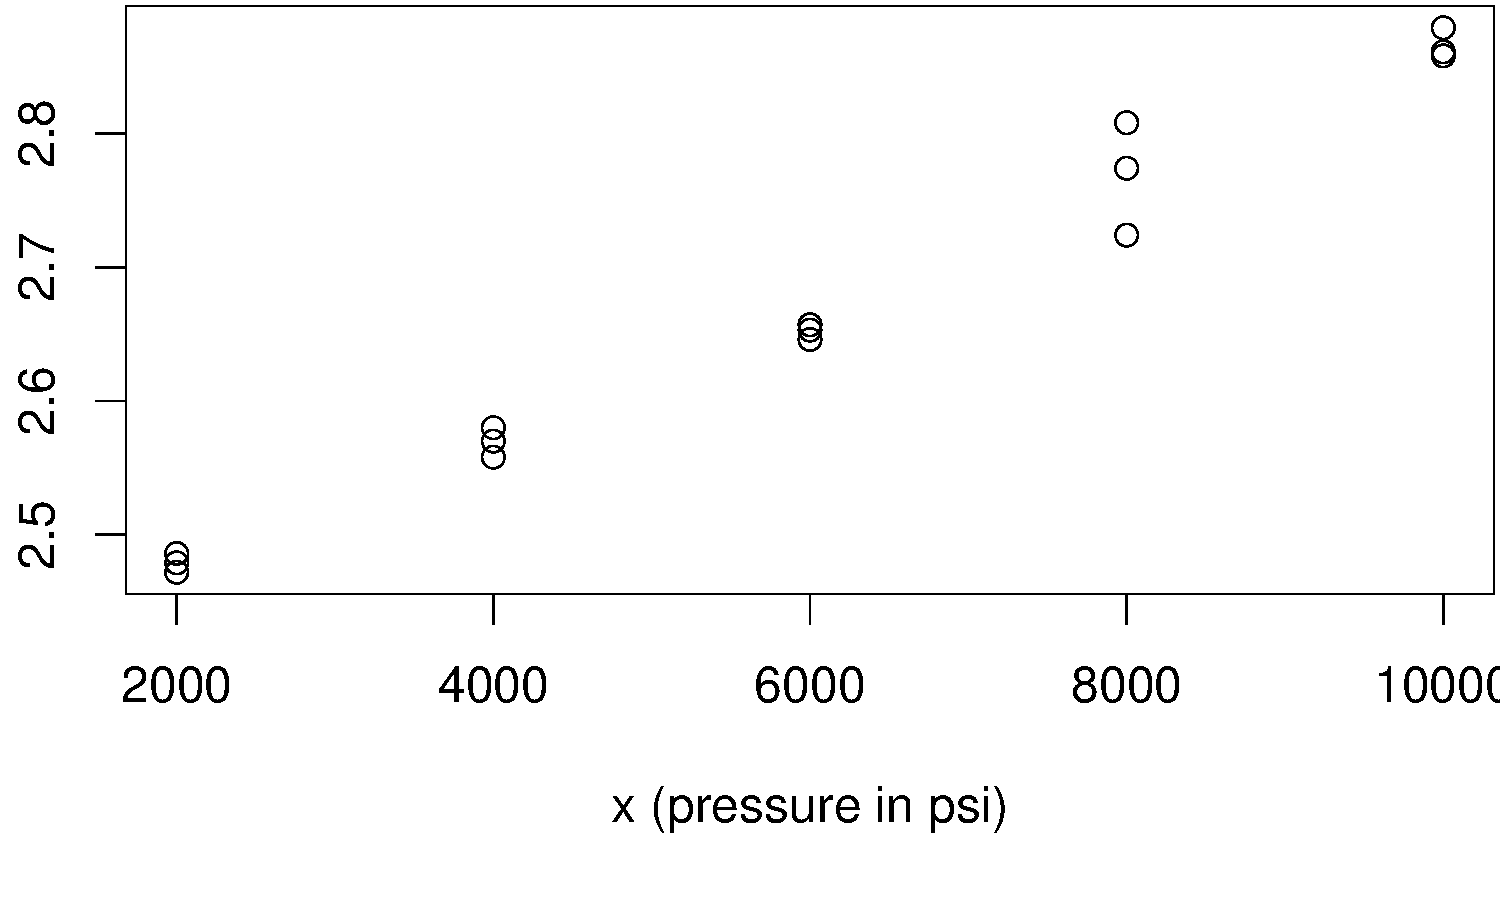
\includegraphics[width=.8\textwidth,height=.6\textheight]{figure/unnamed-chunk-3-1} 

\end{knitrout}
\end{center}
\end{frame}


\begin{frame}[fragile]
\frametitle{}
\begin{center}
\begin{knitrout}
\definecolor{shadecolor}{rgb}{0.969, 0.969, 0.969}\color{fgcolor}
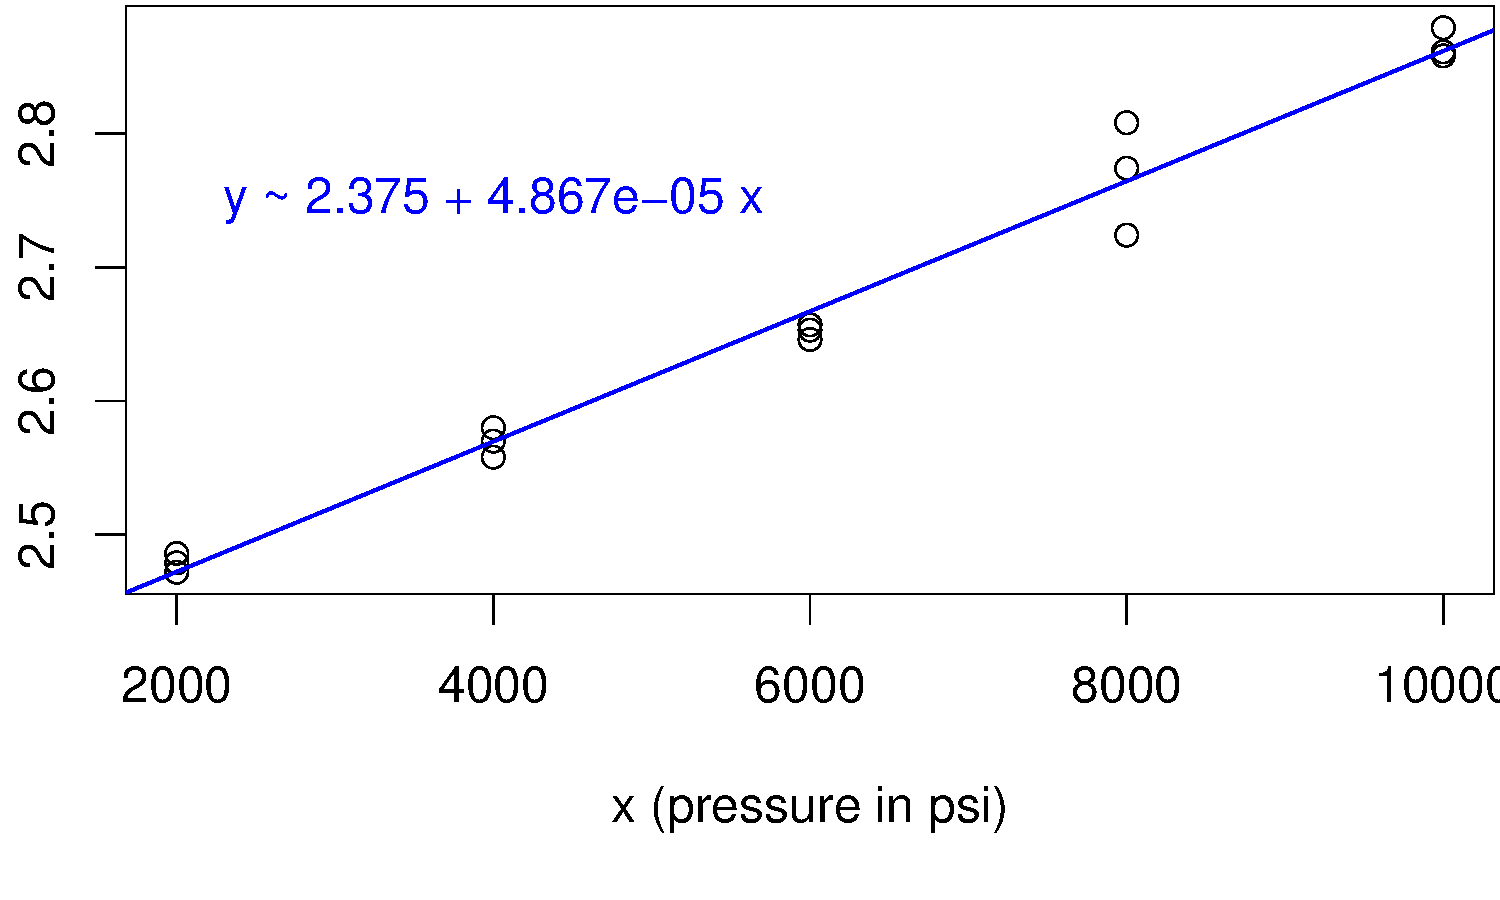
\includegraphics[width=.8\textwidth,height=.6\textheight]{figure/unnamed-chunk-4-1} 

\end{knitrout}
\end{center}

\begin{itemize}
\item The line,  $y \approx 2.375 + 4.867 \times 10^{-5} x$, is the {\bf regression line} fit to the data.
\end{itemize}
\end{frame}

\begin{frame}
\frametitle{Why fit a regression line?}
\begin{enumerate}[1. ]
\item To predict future values of $y$ based on $x$.
\begin{itemize}
\pause \item I.e., a new ceramic under pressure $x = 5000$ psi should have a density of $2.375 + 4.867 \times 10^{-5} \cdot 5000 = 2.618$ g/cc. 
\end{itemize}
\pause \item To characterize the relationship between $x$ and $y$ in terms of strength, direction, and shape.
\begin{itemize}
\pause \item In the ceramics data, density has a strong, positive, linear association with $x$. 
\pause \item On average, the density increases by $4.867 \times 10^{-5}$ g/cc for every increase in pressure of 1 psi.
\end{itemize}
\end{enumerate}
\end{frame}

\begin{frame}
\frametitle{Fitting a linear regression line}
\begin{itemize}
\item For a response variable $y$ and a predictor variable $x$, we declare:
\begin{align*}
y \approx b_0 + b_1 x
\end{align*}
\pause \item and then calculate the intercept $b_0$ and slope $b_1$ using {\bf least squares}.
\begin{itemize}
\pause \item We apply the {\bf principle of least squares}: that is, the best-fit line is given by minimizing the {\bf loss function} in terms of $b_0$ and $b_1$:
\pause \begin{align*}
S(b_0, b_1) = \sum_{i = 1}^n (y_i - \wh{y}_i)^2
\end{align*} 
\item Here, $\wh{y}_i  = b_0 + b_1 x_i$
\end{itemize}
\end{itemize}
\end{frame}


\begin{frame}
\frametitle{\small Minimize $\sum_{i = 1}^n (y_i - \wh{y}_i)^2$ to get the line as close as possible to the points.}
\setkeys{Gin}{width=1\textwidth} 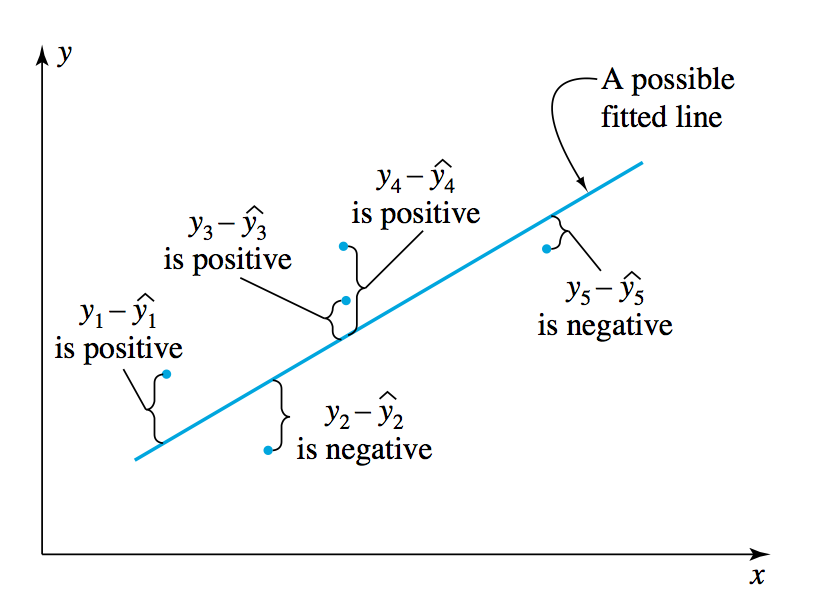
\includegraphics{../../fig/lossfunplot.png}
\end{frame}


\begin{frame}
\frametitle{How to apply least squares to get the regression line}
\begin{itemize}
\item From the principle of least squares, one can derive the {\bf normal equations}:
\pause \begin{align*}
n b_0 + b_1 \sum_{i = 1}^n x_i &= \sum_{i = 1}^n y_i \\
b_0 \sum_{i = 1}^n x_i + b_1 \sum_{i = 1}^n x_i^2 &= \sum_{i = 1}^n x_i y_i 
\end{align*}
\pause \item and then solve for $b_0$ and $b_1$:
\pause \begin{align*}
\color{blue} b_1 = \frac{\sum(x_i - \ov{x})(y_i - \ov{y})}{\sum(x_i - \ov{x})^2} \qquad b_0 = \ov{y}- b_1 \ov{x}
\end{align*}
\end{itemize}
\end{frame}

\begin{frame}[fragile]
\frametitle{Example: plastics hardness data} \small
Eight batches of plastic are made. From each batch one test item is molded. At a given time (in hours), it hardness is measured in units (assume freshly-melted plastic has a hardness of 0 units). The following are the 8 measurements and times.

\begin{minipage}[b]{0.47\linewidth} 
% latex table generated in R 3.5.2 by xtable 1.8-3 package
% Tue Apr 07 11:42:01 2020
\begin{table}[ht]
\centering
\begin{tabular}{rr}
 time & hardness \\ 
  \hline
32.00 & 230.00 \\ 
  72.00 & 323.00 \\ 
  64.00 & 298.00 \\ 
  48.00 & 255.00 \\ 
  16.00 & 199.00 \\ 
  40.00 & 248.00 \\ 
  80.00 & 359.00 \\ 
  56.00 & 305.00 \\ 
  \end{tabular}
\end{table}

\end{minipage}
\begin{minipage}[b]{0.47\linewidth} 
\begin{knitrout}
\definecolor{shadecolor}{rgb}{0.969, 0.969, 0.969}\color{fgcolor}
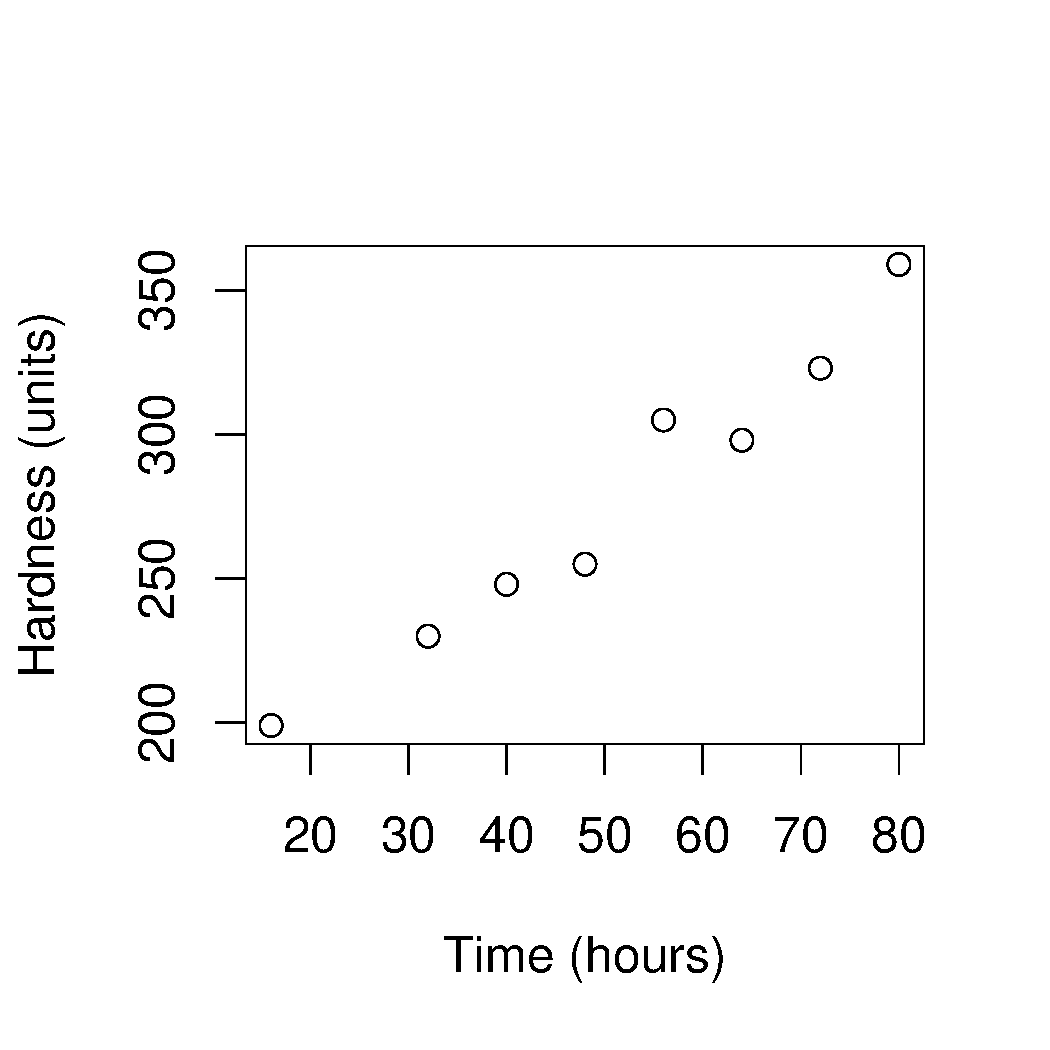
\includegraphics[width=\maxwidth]{figure/unnamed-chunk-6-1} 

\end{knitrout}
\end{minipage}


\end{frame}

\begin{frame}[fragile]
\frametitle{Fitting the line} \scriptsize
\begin{itemize}
\item $\ov{x} = 51$
\item $\ov{y} = 277.125$
% latex table generated in R 3.5.2 by xtable 1.8-3 package
% Tue Apr 07 11:42:01 2020
\begin{table}[ht]
\centering
\begin{tabular}{rrrrrr}
 x & y & $x_i - \ov{x}$ & $y_i - \ov{y}$ & $(x_i - \ov{x})(y_i - \ov{y})$ & $(x_i - \ov{x})^2$ \\ 
  \hline
32.00 & 230.00 & -19.00 & -47.12 & 895.38 & 361.00 \\ 
  72.00 & 323.00 & 21.00 & 45.88 & 963.38 & 441.00 \\ 
  64.00 & 298.00 & 13.00 & 20.88 & 271.38 & 169.00 \\ 
  48.00 & 255.00 & -3.00 & -22.12 & 66.38 & 9.00 \\ 
  16.00 & 199.00 & -35.00 & -78.12 & 2734.38 & 1225.00 \\ 
  40.00 & 248.00 & -11.00 & -29.12 & 320.38 & 121.00 \\ 
  80.00 & 359.00 & 29.00 & 81.88 & 2374.38 & 841.00 \\ 
  56.00 & 305.00 & 5.00 & 27.88 & 139.38 & 25.00 \\ 
  \end{tabular}
\end{table}

\item $\sum (x_i - \ov{x})(y_i - \ov{y}) = 895.38 +  963.38  + \cdots  139.38  =  7765 $
\item $\sum (x_i - \ov{x})^2= 361 +  441  + \cdots  25  =  3192 $
\item $b_1 = \frac{7765}{3192} = 2.43$ 
\item $b_0 = \ov{y} - b_1 \ov{x} = 277.125 - 2.43 \cdot 51 = 153.19$
\end{itemize}
\end{frame}


\begin{frame}[fragile]
\frametitle{Plot the line to check the fit.} \small
\begin{center}
\begin{knitrout}
\definecolor{shadecolor}{rgb}{0.969, 0.969, 0.969}\color{fgcolor}
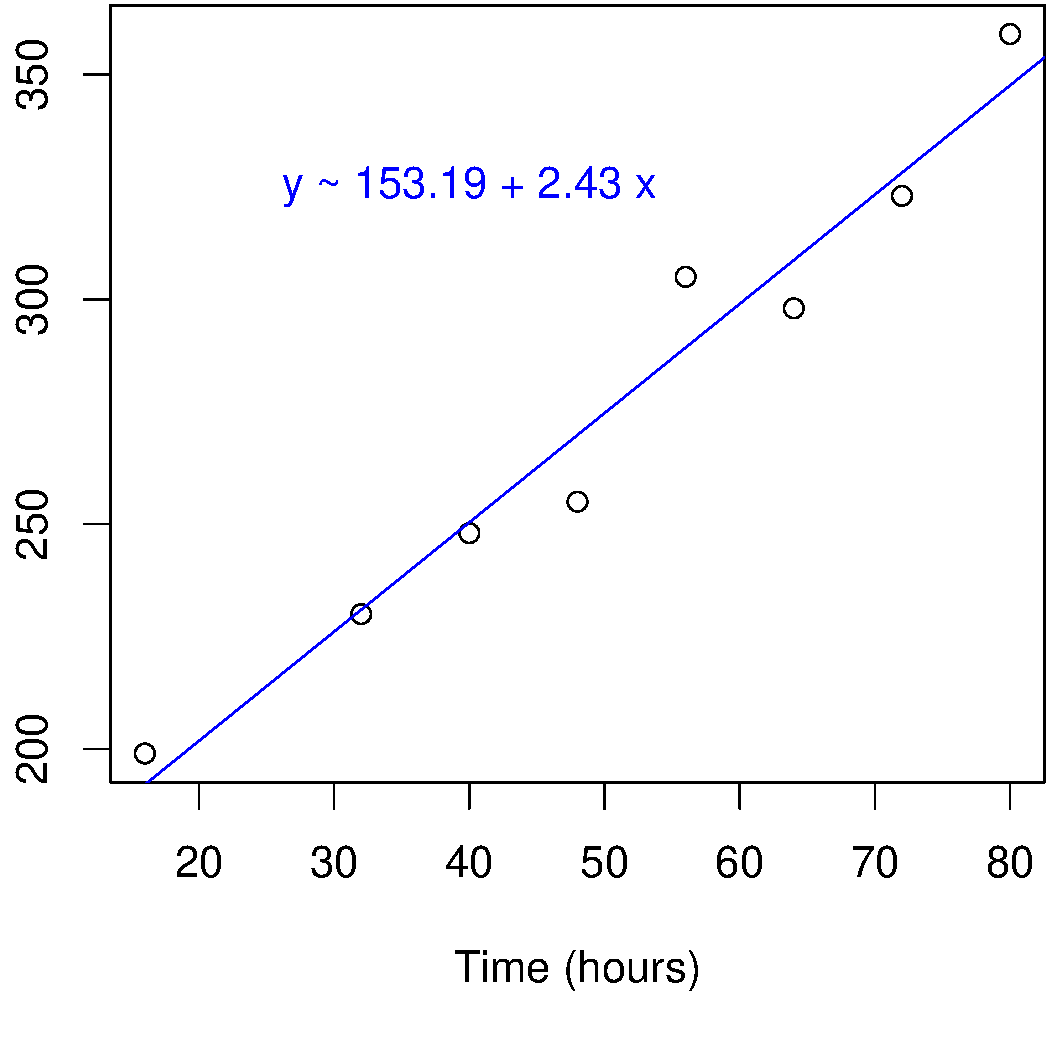
\includegraphics[width=0.8\textwidth,height=0.8\textheight]{figure/unnamed-chunk-8-1} 

\end{knitrout}

\end{center}
\end{frame}

\begin{frame}
\frametitle{Interpret the model terms}
\begin{itemize}
\item $b_1 = 2.43$ means that on average, the plastic hardens 2.43 more units for every additional hour it is allowed to harden.
\pause \item $b_0 = 153.19$ means that if the model is completely true, at the very beginning of the hardening process (time = 0 hours), the plastics had a hardness of 153.19 on average.
\begin{itemize}
\pause \item But we know that the plastics were completely molten at the very beginning, with a hardness of 0.
\pause \item Don't {\bf extrapolate}: i.e., predict $y$ values beyond the range of the $x$ data. 
\end{itemize}
\end{itemize}
\end{frame}


\begin{frame}
\frametitle{Linear correlation: a measure of usefulness}
\begin{itemize}
\item {\bf Linear correlation}: a measure of usefulness of a fitted line, defined by:
\pause \begin{align*}
r = \frac{\sum(x_i - \ov{x})(y_i - \ov{y})}{\sqrt{\sum (x_i - \ov{x})^2 \sum (y_i - \ov{y})^2}}
\end{align*}
\pause \item As it turns out:
\begin{align*}
r = b_1\frac{s_x}{s_y}
\end{align*}
where $s_x$ is the standard deviation of the $x_i$'s and $x_y$ is the standard deviation of the $y_i$'s. 
\end{itemize}
\end{frame}

\begin{frame}
\frametitle{Facts about linear correlation}
\begin{itemize}
\item $-1 \le r \le 1$
\pause \item $r < 0$ means a negative slope, $r > 0$ means a positive slope
\pause \item High $|r|$ means $x$ and $y$ have a strong linear relationship (high correlation), and low $|r|$ implies a weak linear relationship (low correlation).
\end{itemize}

\setkeys{Gin}{width=1\textwidth} 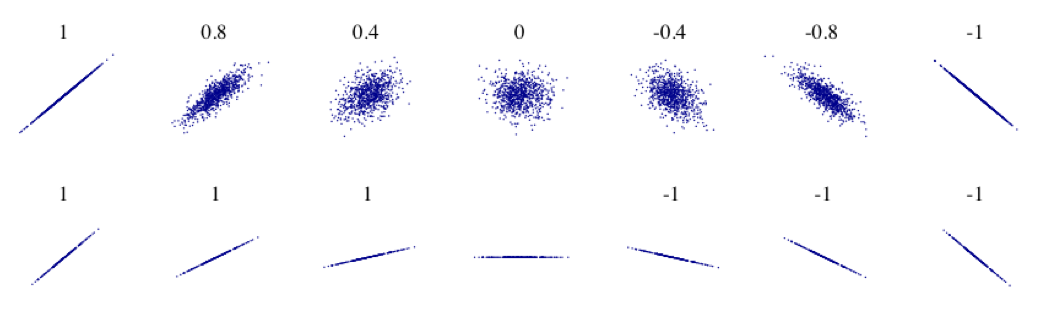
\includegraphics{../../fig/diffcorrs.png}
\end{frame}




\begin{frame}
\frametitle{Coefficient of determination} \scriptsize
\begin{itemize}
\item {\bf Coefficient of determination}: another measure of the usefulness of a fitted line, defined by:
\begin{align*}
R^2 = \frac{\sum(y_i - \ov{y})^2 - \sum(y_i - \wh{y}_i)^2}{\sum(y_i - \ov{y})^2}
\end{align*}
where $\wh{y}_i = b_0 + b_1 x_i$. 
\pause \item Fortunately,
\begin{align*} \color{blue}
R^2 = r^2
\end{align*}
\pause \item Interpretation: $R^2$ is the fraction of variation in the response variable ($y$) explained by the fitted line.
\pause \item Ceramics data: $R^2 = r^2 = 0.9911^2 = 0.9822792$, so  98.227921\% of the variation in density is explained by pressure. Hence, the line is useful for predicting density from pressure.
\pause \item Plastics data: $R^2 = r^2 = 0.9796^2 = 0.9596162$, so  95.961616\% of the variation in hardness is explained by time. Hence, so the line is useful for predicting hardness from time.
\end{itemize}
\end{frame}

\section{Formalizing the Simple Linear Regression Model}

\begin{frame}
\frametitle{The informal simple linear regression model}
\begin{itemize}
\item Up until now, we have looked at fitted lines of the form:
\begin{align*}
y_i = b_0 + b_1 x_i + e_i
\end{align*}
where:
\begin{itemize}
\pause \item $y_1, \ y_2, \ldots, y_n$ are the fixed, observed values of the response variable.
\pause \item $x_1, \ x_2, \ldots, x_n$ are the fixed, observed values of the predictor variable.
\pause \item $b_0$ is the estimated slope of the line based on \emph{sample} data.
\pause \item $b_1$ is the estimated intercept of the line based on \emph{sample} data.
\pause \item $e_i$ is the residual of the $i$'th unit of the sample.
\end{itemize}
\end{itemize}
\end{frame}

\begin{frame}
\frametitle{The formal simple linear regression model} \small
\begin{align*}
Y_i = \beta_0 + \beta_1 x_i + \e_i
\end{align*}
\begin{itemize}
\pause \item $Y_1, \ Y_2, \ldots, Y_n$ are random variables that describe the response.
\pause \item $x_1, \ x_2, \ldots, x_n$ are still fixed, observed values of the predictor variable.
\pause \item $\beta_0$ is a parameter denoting the \emph{true} intercept of the line if we fit it to the population.
\pause \item $\beta_1$ is a parameter denoting the \emph{true} slope of the line if we fit it to the population.
\pause \item $\e_1, \ \e_2, \ldots, \e_n$ are random variables called {\bf error terms}.
\end{itemize}
\end{frame}

\begin{frame}
\frametitle{The formal simple linear regression model} \small

\begin{itemize}
\item We assume:
\begin{align*}
\e_1, \ \e_2, \ldots, \e_n \stackrel{\text{iid}}{\sim} N(0, \sigma^2)
\end{align*}
\pause \item Which means that for all $i$:
\begin{align*}
Y_i \stackrel{\text{iid}}{\sim} N(\beta_0 + \beta_1 x_i, \ \sigma^2)
\end{align*}
\pause \item We often say:
\begin{align*}
\mu_{y \mid x} = \beta_0 + \beta_1 x
\end{align*}
\end{itemize}
\end{frame}

\begin{frame}
\frametitle{The formal simple linear regression model}
\setkeys{Gin}{width=1\textwidth} 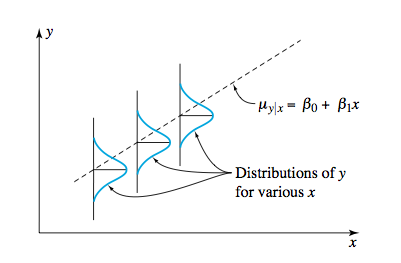
\includegraphics{../../fig/normalsimplereg.png}
\end{frame}

\section{Estimating $\sigma^2$}

\begin{frame}
\frametitle{The line-fitting sample variance}
\begin{itemize}
\item Recall:
\begin{itemize}
\item $\wh{y}_i = b_0 + b_1 x_i $
\pause \item $e_i = y_i - \wh{y}_i$
\end{itemize}
\pause \item The {\bf line-fitting sample variance}, also called {\bf mean squared error} (MSE) is:
\pause \begin{align*}
s_{LF}^2 = \frac{1}{n-2}\sum_i (y_i - \wh{y}_i)^2 = \frac{1}{n-2} \sum_i e_i^2
\end{align*}
\pause and it satisfies:
\pause \begin{align*}
E(s_{LF}^2) = \sigma^2
\end{align*}
\pause \item The line-fitting sample standard deviation is just $s_{LF} = \sqrt{s_{LF}^2}$
\end{itemize}
\end{frame}


\begin{frame}
\frametitle{Example: ceramics} \small
\begin{itemize}
\item A mixture of Al${}_2$O${}_3$, polyvinyl alcohol, and water was prepared, dried overnight, crushed, and sieved to obtain 100 mesh size grains. These were pressed into cylinders at pressures from 2,000 psi to 10,000 psi, and cylinder densities were calculated.
\end{itemize}
\begin{center}
\setkeys{Gin}{width=.38\textwidth} 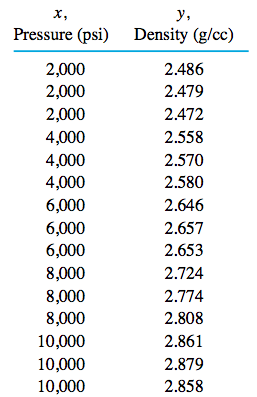
\includegraphics{../../fig/ceramicdat.png}
\end{center}
\end{frame}


\begin{frame}
\frametitle{Example: ceramics}
\setkeys{Gin}{width=1\textwidth} 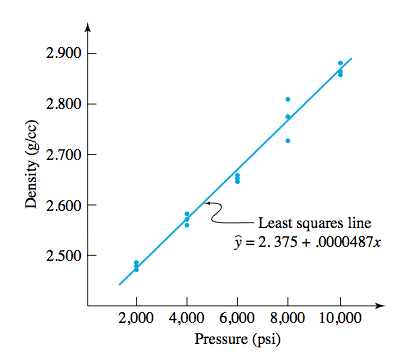
\includegraphics{../../fig/ceramicsplot.png}
\end{frame}


\begin{frame}
\frametitle{Example: ceramics} \scriptsize
\begin{itemize}
\item The fitted least squares line is $\wh{y}_i = 2.375 + 0.0000487 x_i$.
\pause \item The fitted values $\wh{y}_i$ are:
\begin{center}
\setkeys{Gin}{width=.4\textwidth} 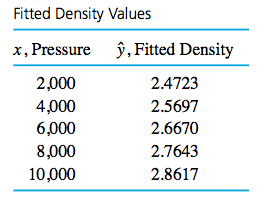
\includegraphics{../../fig/ceramicsfit.png}
\end{center}
\pause \item And $\sum (y_i - \wh{y}_i)^2$ is:
\end{itemize}
\begin{center}
\setkeys{Gin}{width=.8\textwidth} 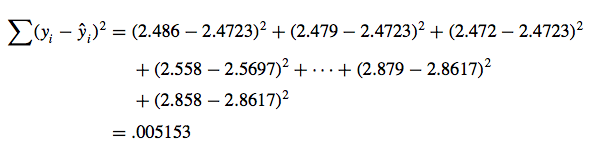
\includegraphics{../../fig/ceramicsyyhat.png}
\end{center}
\begin{itemize}
\pause \item Thus, $s^2_{LF} = \frac{1}{n-2} \sum (y_i - \wh{y}_i)^2 = \frac{1}{15 - 2} \cdot 0.005153 = 0.00396 (g/cc)^2$
\pause \item $s_{LF} = \sqrt{s^2_{LF}} = 0.0199 g/cc$
\end{itemize}
\end{frame}

\section{Standardized residuals}

\begin{frame}
\frametitle{Standardized residuals}
\begin{itemize}
\item Recall that we assume $\e_1, \ldots, \e_n \stackrel{\text{iid}}{\sim} N(0, \sigma^2)$.
\pause \item We also have $E(e_i) = 0$, but because we're \emph{estimating} the slope and intercept instead of using the true slope and intercept,
\pause \begin{align*}
Var(e_j) = \sigma^2 \left ( 1 - \frac{1}{n} - \frac{(x_j-\ov{x})^2}{ \sum_i (x_i - \ov{x})^2} \right )
\end{align*}
\pause \item We don't want $Var(e_j)$ to vary with $j$, so we define the $j$'th {\bf standardized residual}:
\pause \begin{align*}
e_j^* = \frac{e_j}{s_{LF}\sqrt{ 1 - \frac{1}{n} - \frac{(x_j-\ov{x})^2}{ \sum_i (x_i - \ov{x})^2} }}
\end{align*}
which, under our model assumptions, is $\approx N(0,1)$.
\end{itemize}
\end{frame}

\begin{frame}
\frametitle{Example: ceramics} \small
\begin{itemize}
\item Since $\ov{x} = 6000$, we can calculate $\sum(x_i - \ov{x})^2 = 1.2 \times 10^8$.
\end{itemize}
\begin{center}
\setkeys{Gin}{width=.6\textwidth} 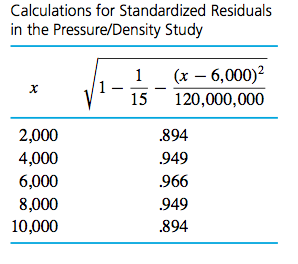
\includegraphics{../../fig/srescalc.png}
\end{center}
\end{frame}


\begin{frame}
\frametitle{Example: ceramics}
\begin{center}
\setkeys{Gin}{width=.7\textwidth} 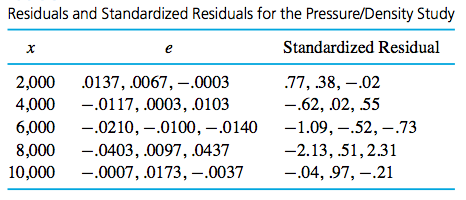
\includegraphics{../../fig/stdres.png}
\end{center}
\end{frame}

\begin{frame}
\frametitle{Example: ceramics}
\begin{center}
\setkeys{Gin}{width=1\textwidth} 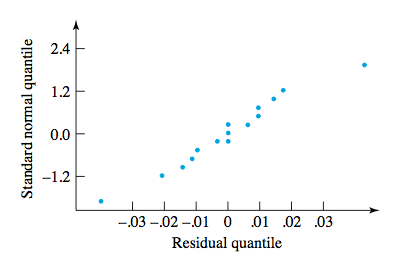
\includegraphics{../../fig/ceramrawres.png}
\end{center}
\end{frame}

\begin{frame}
\frametitle{Example: ceramics}
\begin{center}
\setkeys{Gin}{width=1\textwidth} 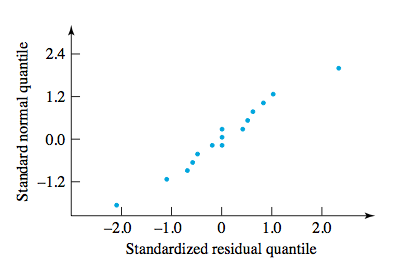
\includegraphics{../../fig/ceramstdres.png}
\end{center}
\end{frame}


\section{Inference for the slope parameter}

\begin{frame}
\frametitle{Inference for the slope parameter}
\begin{itemize}
\item Since $b_1$ was estimated from the data, we can treat it as a random variable.
\pause \item Under the assumptions of the simple linear regression model,
\begin{align*}
b_1 \sim N \left ( \beta_1, \ \frac{\sigma^2}{\sum_i(x_i -\ov{x})^2} \right )
\end{align*}
\pause \item Thus:
\begin{align*}
Z = \frac{b_1 - \beta_1}{\frac{\sigma}{\sqrt{ \sum_i(x_i -\ov{x})^2} }} \sim N(0,1)
\end{align*}
\pause and 
\begin{align*}
T =  \frac{b_1 - \beta_1}{\frac{s_{LF}}{\sqrt{ \sum_i(x_i -\ov{x})^2} }} \sim t_{n-2}
\end{align*}
\end{itemize}
\end{frame}

\begin{frame}
\frametitle{Inference for the slope parameter} \small
\begin{itemize}
\item If we want to test $H_0: \beta_1 = \#$, we can use the test statistic:
\begin{align*}
T = \frac{b_1 - \#}{\frac{s_{LF}}{\sqrt{ \sum_i(x_i -\ov{x})^2} }} \sim t_{n-2}
\end{align*}
\pause which has a $t_{n-2}$ distribution if $H_0$ is true and the model assumptions are true.
\pause \item We can write a two-sided $1 - \alpha$ confidence interval as:
\end{itemize}
\pause \begin{align*}
\left( b_1 - t_{n-2, \ 1 - \alpha/2} \cdot \frac{s_{LF}}{\sqrt{ \sum_i(x_i -\ov{x})^2} }, b_1 + t_{n - 2, 1 - \alpha/2} \cdot \frac{s_{LF}}{\sqrt{ \sum_i(x_i -\ov{x})^2} } \right)
\end{align*}
\begin{itemize}
\pause \item The one-sided confidence intervals are analogous.
\end{itemize}
\end{frame}


\begin{frame}
\frametitle{Example: ceramics} \small
\begin{itemize}
\item I will construct a two-sided 95\% confidence interval for $\beta_1$ ($\alpha = 0.05$).
\pause \item From before, $b_1 = 0.0000487$ g/cc/psi, $\sum_i (x_i - \ov{x})^2 = 1.2 \times 10^8$, and $s_{LF} = 0.0199$.
\pause \item $t_{n -2, \ 1-\alpha/2} = t_{13, \ 0.975} = $ 2.16.
\pause \item The confidence interval is then:
\end{itemize}
\pause \begin{align*}
\left ( 0.0000487 - 2.16 \frac{0.0199}{\sqrt{1.2 \times 10^8}}, \ 0.0000487 + 2.16 \frac{0.0199}{\sqrt{1.2 \times 10^8}}  \right) \\
(0.0000448, \ 0.0000526)
\end{align*}
\begin{itemize}
\pause \item We're 95\% confident that for every unit increase in psi, the density of the next ceramic increases by anywhere between 0.0000448 g/cc and 0.0000526 g/cc.
\end{itemize}
\end{frame}

\begin{frame}
\frametitle{Example: ceramics}
\begin{itemize}
\item In JMP:
\begin{itemize}
\pause \item Open the data in a spreadsheet with:
\begin{itemize}
\pause \item 1 column for $x$
\pause \item 1 column for $y$
\end{itemize}
\pause \item For simple linear regression
\begin{itemize}
\pause \item Click Analyze $\rightarrow$ Fit Y by X
\pause \item Y variable - in Y, Response
\pause \item X variable - in X, Factor
\pause \item Click red triangle - Fit line
\end{itemize}
\end{itemize}
\end{itemize}
\end{frame}

\begin{frame}
\frametitle{Example: ceramics}
\begin{center}
\setkeys{Gin}{width=.48\textwidth} 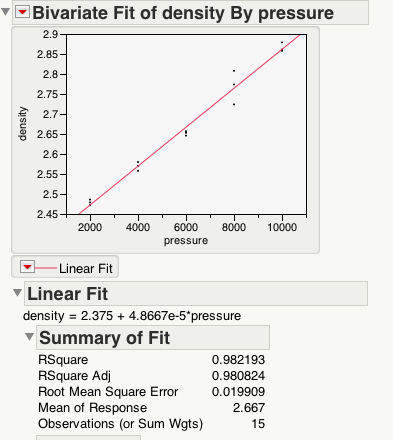
\includegraphics{../../fig/jmpcer1.png}
\setkeys{Gin}{width=.48\textwidth} 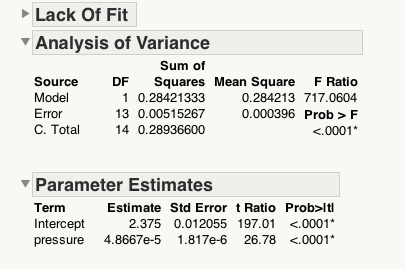
\includegraphics{../../fig/jmpcer2.png}
\end{center}
\end{frame}

\begin{frame}
\frametitle{Example: ceramics}
\begin{center}
\setkeys{Gin}{width=1\textwidth} 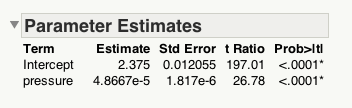
\includegraphics{../../fig/jmpcerparams.png}
\end{center}
\begin{itemize}
\item I can construct the same confidence interval using the JMP output:
\begin{itemize}
\pause \item $b_1 = 4.87 \times 10^{-5}$, $t_{n - 1, 1 - \alpha/2} = 2.16$, $\wh{SD}(b_1) = 1.817 \times 10^{-6}$
\item 
\begin{align*}
&\uncover<3->{(4.87 \times 10^{-5} - 2.16 \cdot 1.817 \times 10^{-6},} \\
 &\uncover<3->{ \qquad 4.87 \times 10^{-5} + 2.16 \cdot 1.817 \times 10^{-6})} \\
&\uncover<4->{= (0.0000448, \ 0.0000526)}
\end{align*}
\end{itemize}
\end{itemize}
\end{frame}


\begin{frame}
\frametitle{Your turn: ceramics}
\begin{center}
\setkeys{Gin}{width=1\textwidth} 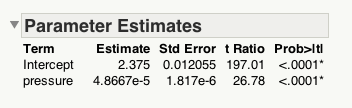
\includegraphics{../../fig/jmpcerparams.png}
\end{center}

\begin{itemize}
\item At $\alpha = 0.05$, conduct a two-sided hypothesis test of $H_0: \beta_1 = 0$ using the method of p-values.
\end{itemize}
\end{frame}

\begin{frame}<handout:\answers>
\frametitle{Answers: ceramics} \small
\begin{enumerate}[1. ]
\item $H_0: \beta_1 = 0$, $H_a: \beta_1 \ne 0$.
\pause \item $\alpha = 0.05$
\pause \item Use the test statistic:
\pause \begin{align*}
T = \frac{b_1 - 0}{\frac{s_{LF}}{\sqrt{\sum(x_i - \ov{x})^2}}} = \frac{b_1}{\wh{SD}(b_1)}
\end{align*}
\pause I assume:
\begin{itemize}
\pause \item $H_0$ is true.
\pause \item The model, $Y_i = \beta_0 + \beta_1 x_i + \e_i$ with errors $\e_i \sim$ iid $N(0, \sigma^2)$, is correct.  
\end{itemize}
Under these assumptions, $T \sim t_{n - 2} = t_{15 - 2} = t_{13}$
\end{enumerate}
\end{frame}


\begin{frame}<handout:\answers>
\frametitle{Answers: ceramics} \small
\begin{enumerate}
\setcounter{enumi}{3}
\item  Observed test statistic:
\begin{align*}
\uncover<2->{t} & \uncover<2->{= \frac{4.87 \times 10^{-5}}{1.817 \times 10^{-6}}} \uncover<3->{= 26.80 \quad \text{(``t Ratio" in JMP output)}} \\
\uncover<4->{\text{p-value}} & \uncover<4->{= P(|t_{13}| > |26.8|)} \uncover<5->{ = P(t_{13} > 26.8) + P(t_{13} < - 26.8)} \\
&\uncover<6->{< 0.0001 \quad (\text{"Prob$>|t|$" in JMP output})}
\end{align*}
\uncover<7->{\item With a p-value $< 0.0001 < 0.05 = \alpha$, we reject $H_0$ and conclude $H_a$.}
\uncover<8->{\item There is overwhelming evidence that the true slope of the line is different from 0.}
\end{enumerate}
\end{frame}

\section{F-test and ANOVA table}
\begin{frame}
\frametitle{ANOVA method for testing $H_0: \beta_1 = 0,\, H_a: \beta_1 \neq 0$}
\begin{itemize}
\item Another method for testing $H_0: \beta_1 = 0,\, H_a: \beta_0 \neq 0$ is the ``ANalysi Of VAriance'' (ANOVA) method.
\item Fact: the Total Sum of Squares can be decomposed into Error Sum of Squares and Regression Sum of Squares. 
\[\underset{SSTol}{\sum_{i=1}^n(y_i - \bar{y})^2} = \underset{SSE}{\sum_{i=1}^n (y_i - \hat{y}_i)^2} + \underset{SSR}{\sum_{i=1}^n (\hat{y}_i - \bar{y})}\]

\item Under the assumptions of SLR model, and assuming $H_0: \beta_1 = 0$ is true, the test statistic
\[F = \frac{SSR/1}{SSE/(n-2)}\]
has a $F_{1, n-2}$ distribution. (Reiview F distribution in {\color{blue} ch5part5\_Mar\_3.pdf}.)
\end{itemize}
\end{frame}

\begin{frame}
\frametitle{ANOVA method for testing $H_0: \beta_1 = 0,\, H_a: \beta_1 \neq 0$}
\begin{itemize}
\item We reject $H_0: \beta_1 = 0$ in favor of $H_a: \beta_1 \neq 0$ when the test statistic $F$ is large. So the p-value is
\[P(F_{1, n-2} > \mbox{observed $F$})\]

\item
In fact, the square of the t statistic for testing $H_0 : \beta_1 = 0$ is
\[T^2 = \left(\frac{b_1 - 0}{\frac{s_{LF}}{\sqrt{\sum (x_i - \bar{x})^2}}}\right) = \frac{SSR/1}{SSE/(n-2)} = F\]
which has an $F_{1, n-2}$ distribution if $H_0$ is true and tends to be large if $H_0$ is false. So counting large $F$ as evidence against $H_0$ in favor of $H_a: \beta_1 \neq 0$ is a sensible significance testing method.
\end{itemize}
\end{frame}

\begin{frame}
\frametitle{ANOVA table}
Calculations in the ANOVA method can be summarized in the ANOVA table:

\vspace{2em}

\scriptsize
\begin{tabular}{lllll}
Source & SS & df & MS & F\\ \hline
Regression & SSR & 1 & MSR = SSR/1 & F = MSR/MSE\\
Error & SSE & $n-2$ & MSE = SSE/$(n-2)$ & \\ \hline
Total & SSTot & $n-1$ & &
\end{tabular}
\end{frame}

\begin{frame}
\frametitle{Example: Ceramics}
\begin{center}
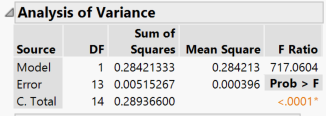
\includegraphics[width = 0.9\textwidth]{../../fig/ch9SLR_ceramics_ANOVA.PNG}
\end{center}
\begin{itemize}
\item
The p-value in the F-test is very small. So we reject $H_0$. 
\item There is significant evidence that the true slope is different from 0.
\end{itemize}
\end{frame}



\end{document}
